\chapter{Dihomotopy equivalences and the fundamental category}
\label{chap:diheq}

With this chapter, we start our study of directed spaces using tools from algebraic topology. We first investigate dihomotopy equivalences. In classical algebraic topology, homotopy equivalences are a way to describe that two topological spaces can be continuously deformed into each other. For directed spaces, an analogue would be that two d-spaces can be continuously deformed into each other, using transformations that preserve somehow directedness. We will see that there are several possible way to express the preservation of directedness.

Classically, homotopy equivalences are defined as continuous functions that are invertible up to homotopy. Much as homotopy of paths, homotopy of functions can be defined either with classical homotopy, that is, function from $X\times [0,1]$ to $Y$, or as a function from $X$ to the space of paths $P(Y)$. There is an analogue of this idea for directed algebraic topology: one can defined several notions of dihomotopies of dimaps by either as dimaps $X\times I$ to $Y$, with $I$ being a directed structure of $[0,1]$, or as a particular function from $X$ to a sub-space of the space of dipaths of $Y$. There will be a correspondence between structures of the segments as seen in Chapter 2 and known classes of dipaths. We will see this in Section \ref{sec:eqexfr}

In Section \ref{sec:geovi}, we have seen the fundamental category of a d-space, which is a summary of the dihomotopy structure of dipaths of this d-space. We would like it to be an invariant of dihomotopy equivalence. In the classical case, the fundamental groupoid of a space is an invariant modulo homotopy equivalence, meaning that a homotopy equivalence induces an equivalence of categories between fundamental groupoids. As observed in \cite{grandis09}, in the directed case, this is strictly true only for reversible equivalences, that is, dihomotopy equivalences defined with $\overleftrightarrow{[0,1]}$ as directed structure on the segment, not for directed equivalences, that is, dihomotopy equivalences defined with $\revseg$ as directed structure. We will see this in Section \ref{subsec:funcla}. The crucial observation is that it fails only because too few morphisms in the fundamental category are isomorphisms. The idea is then to invert some morphisms to make the fundamental category an invariant of other types of dihomotopy equivalences. This process of inverting morphisms of a category is called localization. We will then see in Section \ref{subsec:grpi}, that a directed equivalence induces an equivalence of categories between groupoidifications of the fundamental categories, that is, the categories obtained by inverting every morphism in the fundamental category.

However, the groupoidification is a bit disappointing: the functor from a category to its groupoidification is not faithful, meaning that we lose information from the category. In particular, even when the category is not cancellative, groupoidification is still a groupoid and so cancellative. Consequently, groupoidification loses cancellative behaviors. Following ideas from \cite{goubault07} on the category of components, we will look in Section \ref{sec:inecomp} at a better localization of the fundamental category: we will localize at morphisms that behave like isomorphisms, meaning that they must induces isomorphisms of Hom-sets by composition, and a condition similar to closure under pullbacks and pushouts, the Ore conditions, which makes our framework different from that of Goubault et al. They will be called inessential morphisms. We will see that this set of morphisms has many nice properties: it has the 2-out-of-6 property (Section \ref{subsec:inemor}), it has a calculus of right and left fractions, it is saturated (Section \ref{subsec:calfra}). In particular, a calculus of right and left fractions allows us to localize a category at those inessential morphisms nicely, forming the category of components, following the terminology from \cite{goubault07}. Finally, we prove in Section \ref{subsec:equiquo} that the category of components is equivalent to a quotient (which allows one in some cases to do computations) for a larger class of categories than in \cite{goubault07}, namely for categories whose subcategory of inessential morphisms has a selection.

\section{Existing frameworks}
\label{sec:eqexfr}
	\subsection{Non directed case}
	\label{subsec:ndc}
	
	We have seen the notion of homotopies between paths, defined as a path in the space of paths. This can be extended to general functions. A \textbf{homotopy} between continuous functions $\map{f,g}{X}{Y}$ is continuous function $\map{H}{X}{\pathsp{Y}}$ such that $x \mapsto H(x)(0)$ is equal to $f$ and $x \mapsto H(x)(1)$ is equal to $g$. As argued in the previous chapter, there is another way (which is the usual way that you can find in textbooks, such as \cite{hatcher02}) to define homotopy between functions. Let us call a \textbf{classical homotopy} between $\map{f,g}{X}{Y}$, a continuous function $\map{K}{X\times[0,1]}{Y}$ such that $x \mapsto K(x,0)$ is equal to $f$ and $x \mapsto K(x,1)$ is equal to $g$. Using one or the other is the same:
	
	\begin{prop}
	There is a homotopy between two functions if and only if there is a classical homotopy between them.
	\end{prop}
	
	\begin{proof}
	Let us first assume that there is a homotopy $\map{H}{X}{\pathsp{Y}}$. We construct the classical homotopy $\map{K}{X\times[0,1]}{Y}$ which maps $(x,t)$ to $H(x)(t)$. The only thing to prove is that it is continuous. Let $V$ be an open set of $Y$. Let us prove that $K^{-1}(V)$ is open in $X\times[0,1]$. Let $(x,t) \in K^{-1}(V)$. This means that $H(x)(t) \in V$, that is, $t \in H(x)^{-1}(V)$. Since $H(x)$ is continuous, $H(x)^{-1}(V)$ is an open set of $[0,1]$ which contains $t$. Since $[0,1]$ is compact and so locally compact, there are an open set $W$ and a compact $K$ of $[0,1]$ such that $t \in W \subseteq K \subseteq H(x)^{-1}(V)$. We consider then the open set $[K,V] = \{\gamma \mid \gamma(K)\subseteq V\}$ of $\pathsp{Y}$. By construction of $K$, $x \in H^{-1}([K,V])$ and since $H$ is continuous, $H^{-1}([K,V])$ is open in $X$. Then $H^{-1}([K,V])\times W$ is an open set of $X\times [0,1]$, which contains $(x,t)$ and which is contained in $K^{-1}(V)$.
	
	Reciprocally, let us assume that there is a classical homotopy $\map{K}{X\times [0,1]}{Y}$. We construct the homotopy $\map{H}{X}{\pathsp{Y}}$ which maps $x$ to $t \mapsto K(x,t)$. Given a open set $[K,V]$ of $\pathsp{Y}$, let $x \in H^{-1}([K,V])$. Since $V$ is open in $Y$ and $K$ is continuous, $K^{-1}(V)$ is open in $X\times[0,1]$. For every $t \in K$, since $(x,t) \in K^{-1}(V)$, there is $U_t$ open set of $X$ and $W_t$ open set of $[0,1]$ such that $(x,t) \in U_t\times W_t \subseteq K^{-1}(V)$. Since $K$ is compact and $(W_t)_{t\in K}$ forms a covering of $K$ with open sets, there is a finite subcovering $(W_t)_{t \in Q}$ of $K$. Define $U = \bigcap\limits_{t\in Q} U_t$. This is an open set of $X$ which contains $x$ and such that $U\times K \subseteq K^{-1}(V)$, that is $U \subseteq H^{-1}([K,V])$.
	\end{proof}
	
	In either case, we say that $f$ and $g$ are \textbf{homotopic} if there is a (classical) homotopy between them. The idea is that two homotopic maps are equal up to continuous deformations. In algebraic topology, we are interested in equivalences of spaces up to continuous deformations. This will be defined using \textbf{homotopy equivalences}: we say that a continuous function $\map{f}{X}{Y}$ is a homotopy equivalence if there is a continuous function $\map{g}{Y}{X}$ such that $f\circ g$ and $g\circ f$ are homotopic to identities. This means essentially that $f$ is a homeomorphism up to continuous deformations. We say that two spaces are \textbf{homotopically equivalent} if there is a homotopy equivalence between them.
	
	Let us illustrate this on examples.
	\begin{enumerate}
		\item Consider two discrete spaces $X$ and $Y$, that is, whose open sets are all subsets. $X$ and $Y$ are homotopically equivalent if and only if they are in bijection.
		\item Every two cubes $\Box_n$ and $\Box_p$ are homotopically equivalent. Since homotopy equivalences are closed under composition, it is sufficient to prove that $\Box_n$ is equivalent to $\Box_0$, that is, a point space. The constant continuous function from $\Box_n$ to $\{(0, \ldots, 0)\}$ is inverse of the inclusion modulo homotopy. When a space is homotopically equivalent to a point space, we say that it is \textbf{contractible}. Contractible spaces are, in some way, the simplest spaces that we may consider.
		\item The circle is not contractible: the intuition is that ``holes'' must be conserved by homotopy equivalences. That is one of the main idea in algebraic topology, ``holes'' give algebraic information of the space which are invariant of homotopy equivalences, and are ``obstructions'' to contractibility.
		\item The circle, the boundary of a square and the annulus are all homotopically equivalent.
			\begin{center}
				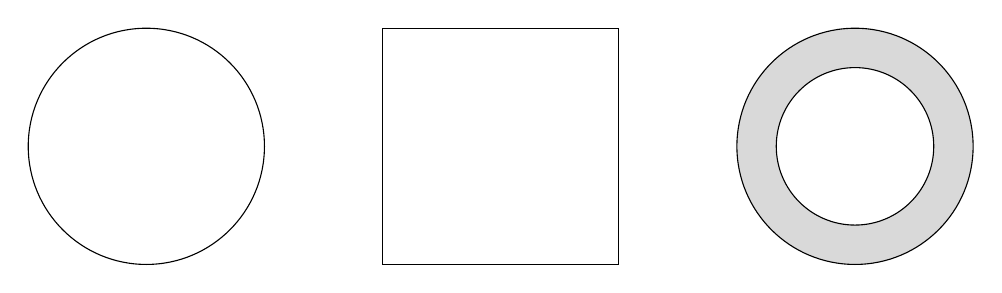
\begin{tikzpicture}[auto,scale = 1]

		\draw (0,0) circle (1.5cm);
		\draw (3,-1.5) -- (6,-1.5) -- (6,1.5) -- (3,1.5) -- cycle;
		\draw [fill=gray, fill opacity = 0.3,even odd rule] (9,0) circle (1.5) (9,0) circle (1);
		
\end{tikzpicture}
			\end{center}
	\end{enumerate} 
	
	Since homotopies are closed under compositions, that is, if $f_1$ is homotopic to $f_2$ and $g_1$ is homotopic to $g_2$, then $g_1\circ f_1$ is homotopic to $g_2\circ f_2$, one can quotient $\topo$ by homotopy. We call \textbf{homotopy category} of $\topo$, the category $\hotop$ whose objects are topological spaces and whose morphisms are homotopy classes of continuous functions. Isomorphisms in $\hotop$ are precisely the homotopy classes of homotopy equivalences.
	
	\subsection{Several extensions}

	
	As we have seen, there are several possible directed structures on the segment $[0,1]$, each of which defining a notion of classical dihomotopy: for $I \in \{\overline{[0,1]}, \dirseg, \dirsegrev, \revseg, \overleftrightarrow{[0,1]}\}$, a \textbf{$I$-dihomotopy} is a dimap $\map{K}{X\times I}{Y}$. The existence of a $I$-dihomotopy between two dimaps is an equivalence relation for $I \in \{\overline{[0,1]}, \revseg, \overleftrightarrow{[0,1]}\}$ but not for $I \in \{\dirseg, \dirsegrev\}$. We then say that two dimaps are \textbf{$I$-dihomotopic} if there is a zig-zag of $I$-dihomotopies between them, that is, there are dimaps $f_0 = f$, $f_1$, \ldots, $f_n$, $f_{n+1} = g$, and $I$-dihomotopies $K_1$, \ldots, $K_{n+1}$ with for every $i$, $x \mapsto K_i(x,0)$ equal to $f_{i-1}$ and $x \mapsto K_i(x,1)$ equal to $f_i$, or vice versa. We say that a dimap is a \textbf{$I$-dihomotopy equivalence} if it is invertible up to $I$-dihomotopy and we say that two d-spaces are \textbf{$I$-dihomotopically equivalent} if there is a $I$-dihomotopy equivalence between them. 
	
	Among those five notions of dihomotopy/dihomotopy equivalence, three of them are of particular interest because they are equivalent to the existence of a continuous function $H$ from $X$ to a subspace of $\pathsp{Y}$ such that for every $t \in [0,1]$, $x \mapsto H(x)(t)$ is a dimap. Only the subspace involved changes:
	\begin{itemize}
		\item if $I = \overline{[0,1]}$, we consider the whole space of paths $\pathsp{X}$. This seems not to be considered in the literature, mainly because it does not sufficiently use directedness. We may call them \textbf{undirected dihomotopies/equivalences}.
		\item if $I =  \dirseg$, we consider the space of dipaths $\dip{X}$. It is the main notion used in \cite{grandis09}. It is called dihomotopy equivalence there. The main idea is that everything is defined using only $\dirseg$ as structure on the segment. We will call it \textbf{directed dihomotopies/equivalences}.
		\item if $I = \revseg$, we consider the space of reversible dipaths $\rev{X}$, that is, dipaths $\gamma$ such that $\gamma^{-1}$ is also a dipath. Being equivalent in this case is really strong since in general there are not many reversible dipaths. For example, in po-spaces seen as d-spaces, the only reversible dipaths are constant paths, and being equivalent then means being dihomeomorphic (that is, isomorphic in the category $\dtop$). This equivalence is called \textbf{reversible dihomotopies/equivalences} \cite{grandis09}.
	\end{itemize}
	
%	\subsection{Other formalisms}
%	
%	fouiller un peu chez Sanjeevi et Martin
	
	\subsection{Examples of $I$-dihomotopy equivalences}
	\label{subsec:exa}


	\begin{enumerate}
		\item Let us first look at the different directed structures of the segment and when they are equivalent to a point space. Note $<$ the order on the set $S = \{\overline{[0,1]},\dirseg,\revseg\}$ such that:
		$$\overline{[0,1]} < \dirseg < \revseg.$$
		
		\begin{prop}
			For every $I, J \in S$, $I$ is $J$-dihomotopically equivalent to a point space if and only if $J \leq I$.
		\end{prop}
		
		The ``if'' part comes from the fact that the constant map from $I$ to $\{0\}$ is inverse modulo $J$-dihomotopy to the inclusion from $\{0\}$ to $I$. The ``only if'' part comes from the fact that if $J > I$, then there is no dimap $\gamma$ from $J$ to $I$ such that $\gamma(0) = 0$ and $\gamma(1) = 1$. For example, in the case where $I = \dirseg$ and $J = \revseg$, this means that there is no dipath from $1$ to $0$ in $\dirseg$.
		
		More generally, the cube $I^k$ is $J$-dihomotopically equivalent to a point if and only if $J \leq I$ by the same arguments.
		

		\item Let us look now at the following two d-spaces:
			\begin{center}
				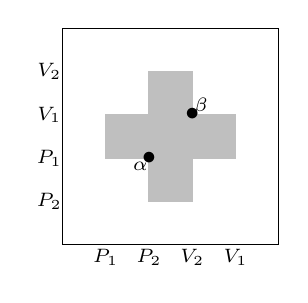
\begin{tikzpicture}[auto,scale = 0.55]
\draw (0,0) rectangle (5,5);
\draw [fill = gray!50,draw = gray!50] (1,2) rectangle (4,3);
\draw [fill = gray!50,draw = gray!50] (2,1) rectangle (3,4);
\node (P1a) at (1,-0.3) {\scriptsize{$P_1$}};
\node (P1b) at (2,-0.3) {\scriptsize{$P_2$}};
\node (P2b) at (-0.3,1) {\scriptsize{$P_2$}};
\node (P2a) at (-0.3,2) {\scriptsize{$P_1$}};
\node (V1b) at (3,-0.3) {\scriptsize{$V_2$}};
\node (V1a) at (4,-0.3) {\scriptsize{$V_1$}};
\node (V2a) at (-0.3,3) {\scriptsize{$V_1$}};
\node (V2b) at (-0.3,4) {\scriptsize{$V_2$}};
\node (dead) at (2,2) {$\bullet$};
\node (ina) at (3,3) {$\bullet$};
\node (al) at (1.8,1.8) {\scriptsize{$\alpha$}};
\node (be) at (3.2,3.2) {\scriptsize{$\beta$}};
\end{tikzpicture}
\quad\quad\qquad
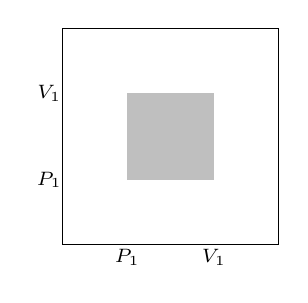
\begin{tikzpicture}[auto,scale = 0.55]
\draw (0,0) rectangle (5,5);
\draw [fill = gray!50,draw = gray!50] (1.5,1.5) rectangle (3.5,3.5);
\node (P1a) at (1.5,-0.3) {\scriptsize{$P_1$}};
\node (P2a) at (-0.3,1.5) {\scriptsize{$P_1$}};
\node (V1a) at (3.5,-0.3) {\scriptsize{$V_1$}};
\node (V2a) at (-0.3,3.5) {\scriptsize{$V_1$}};
\end{tikzpicture}
			\end{center}
		
		They are geometric realization of PV-programs. They are subspaces of $[0,1]^2$ (in white) in which we have carved small rectangles (in grey). Their dipaths are component-wise monotonous paths. The left one is called the \textbf{Swiss flag} (SF) and the right one the \textbf{squared annulus} (SA). First, those two d-spaces are not reversibly equivalent since they are po-spaces and they are not isomorphic because of the local maximum $\alpha$ (resp. local minimum $\beta$). From a computer science point of view $\alpha$ (resp. $\beta$) corresponds to a deadlock (resp. an inaccessible state). On the other hand, they are directedly equivalent (and so undirectedly equivalent). There are a dimap from SF to SA (whose image is depicted in light grey on the left below) and a dimap from SA to SF (whose image is depicted in light grey on the right below), which are inverse to each other up to directed dihomotopies.
			\begin{center}
				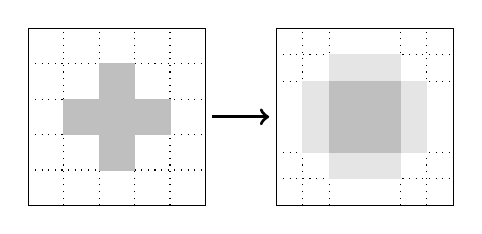
\begin{tikzpicture}[auto,scale = 0.45]
\draw (0,0) rectangle (5,5);
\draw [dotted] (1,0) -- (1,5);
\draw[dotted] (2,0) -- (2,5);
\draw[dotted] (3,0) -- (3,5);
\draw[dotted] (4,0) -- (4,5);
\draw [dotted] (0,1) -- (5,1);
\draw[dotted] (0,2) -- (5,2);
\draw[dotted] (0,3) -- (5,3);
\draw[dotted] (0,4) -- (5,4);
\draw [fill = gray!50,draw = gray!50] (1,2) rectangle (4,3);
\draw [fill = gray!50,draw = gray!50] (2,1) rectangle (3,4);
\draw[->,very thick] (5.2,2.5) -- (6.8,2.5);
\draw (7,0) rectangle (12,5);
\draw [dotted] (7.75,0) -- (7.75,5);
\draw[dotted] (8.5,0) -- (8.5,5);
\draw[dotted] (10.5,0) -- (10.5,5);
\draw[dotted] (11.25,0) -- (11.25,5);
\draw [dotted] (7,0.75) -- (12,0.75);
\draw[dotted] (7,1.5) -- (12,1.5);
\draw[dotted] (7,3.5) -- (12,3.5);
\draw[dotted] (7,4.25) -- (12,4.25);
\draw[fill = gray!20,draw=gray!20] (7.75,1.5) rectangle (11.25,3.5);
\draw[fill = gray!20,draw=gray!20] (8.5,0.75) rectangle (10.5,4.25);
\draw [fill = gray!50,draw = gray!50] (8.5,1.5) rectangle (10.5,3.5);
\end{tikzpicture}
\quad\quad\quad
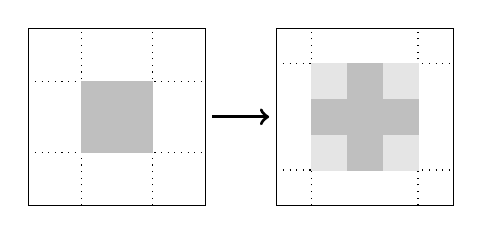
\begin{tikzpicture}[auto,scale = 0.45]
\draw (0,0) rectangle (5,5);
\draw [dotted] (3.5,0) -- (3.5,5);
\draw[dotted] (1.5,0) -- (1.5,5);
\draw [dotted] (0,1.5) -- (5,1.5);
\draw[dotted] (0,3.5) -- (5,3.5);
\draw [fill = gray!50,draw = gray!50] (1.5,1.5) rectangle (3.5,3.5);
\draw[->,very thick] (5.2,2.5) -- (6.8,2.5);
\draw (7,0) rectangle (12,5);
\draw [dotted] (11,0) -- (11,5);
\draw[dotted] (8,0) -- (8,5);
\draw [dotted] (7,1) -- (12,1);
\draw[dotted] (7,4) -- (12,4);
\draw [fill = gray!20,draw = gray!20] (8,1) rectangle (11,4);
\draw[fill = gray!50,draw=gray!50] (8,2) rectangle (11,3);
\draw[fill = gray!50,draw=gray!50] (9,1) rectangle (10,4);
\end{tikzpicture}
			\end{center}	
		
		
		\item We will see later that the matchbox $\matchbox$ is not reversibly equivalent to a point. The argument will use the fundamental category. We prove now that it is directedly equivalent to a point. Since we have seen that the square $\dirseg^2$ is directedly equivalent to a point, it is enough to prove that $\matchbox$ is equivalent to its upper face. It is easy to prove that the injection $\iota$ of the upper face into the matchbox is inverse modulo directed dihomotopy to the projection  $p$ of the matchbox on its upper face. In one direction, $p\circ\iota$ is equal to identity, in the other direction a dihomotopy from identity to $\iota\circ p$ is given by this picture:
			\begin{center}
				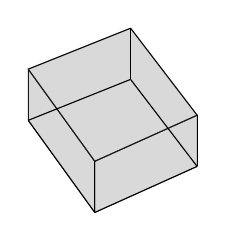
\begin{tikzpicture}[auto,scale = 0.65]
		\coordinate (A) at (0,0);
		\coordinate (B) at (2,0.9);
		\coordinate (C) at (-1.3,1.8);
		\coordinate (D) at (0.7,2.6);
		\coordinate (A') at (0,1);
		\coordinate (B') at (2,1.9);
		\coordinate (C') at (-1.3,2.8);
		\coordinate (D') at (0.7,3.6);
		\draw (B) -- (B');
		\draw (A') -- (B');
		\draw (C) -- (C');
		\draw (A') -- (C');
		\draw (B') -- (D');
		\draw (C') -- (D');
		\draw [fill = gray,draw = black,opacity = 0.3] (A) -- (B) -- (B') -- (A') -- (A);
		\draw [fill = gray,draw = black,opacity = 0.3] (A) -- (C) -- (C') -- (A') -- (A);
		\draw [fill = gray,draw = black,opacity = 0.3] (A') -- (B') -- (D') -- (C') -- (A');
		\draw(A) -- (B);
		\draw (A) -- (C);
		\draw (B) -- (D);
		\draw (C) -- (D);
		\draw (D) -- (D');
		\draw (A) -- (A');
		\end{tikzpicture}
		\quad\quad\quad
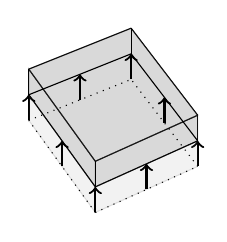
\begin{tikzpicture}[auto,scale = 0.65]
		\coordinate (A'') at (0,0);
		\coordinate (B'') at (2,0.9);
		\coordinate (C'') at (-1.3,1.8);
		\coordinate (D'') at (0.7,2.6);
		\coordinate (A) at (0,0.5);
		\coordinate (B) at (2,1.4);
		\coordinate (C) at (-1.3,2.3);
		\coordinate (D) at (0.7,3.1);
		\coordinate (A') at (0,1);
		\coordinate (B') at (2,1.9);
		\coordinate (C') at (-1.3,2.8);
		\coordinate (D') at (0.7,3.6);
		\draw (B) -- (B');
		\draw (A') -- (B');
		\draw (C) -- (C');
		\draw (A') -- (C');
		\draw (B') -- (D');
		\draw (C') -- (D');
		\draw [fill = gray,draw = black,opacity = 0.3] (A) -- (B) -- (B') -- (A') -- (A);
		\draw [fill = gray,draw = black,opacity = 0.3] (A) -- (C) -- (C') -- (A') -- (A);
		\draw [fill = gray,draw = black,opacity = 0.3] (A') -- (B') -- (D') -- (C') -- (A');
		\draw(A) -- (B);
		\draw (A) -- (C);
		\draw (B) -- (D);
		\draw (C) -- (D);
		\draw (D) -- (D');
		\draw (A) -- (A');
		\draw[<-, thick] (B) -- (B'');
		\draw[dotted] (A'') -- (B'');
		\draw[<-, thick] (C) -- (C'');
		\draw[dotted] (A'') -- (C'');
		\draw[dotted] (B'') -- (D'');
		\draw[dotted] (C'') -- (D'');
		\draw [fill = gray,draw = black,opacity = 0.1] (A'') -- (B'') -- (B) -- (A) -- (A'');
		\draw [fill = gray,draw = black,opacity = 0.1] (A'') -- (C'') -- (C) -- (A) -- (A'');
		\draw[<-, thick] (D) -- (D'');
		\draw[<-, thick] (A) -- (A'');
		\draw[->,thick] (-0.65,0.9) -- (-0.65,1.4);
		\draw[->,thick] (1,0.45) -- (1,0.95);
		\draw[->,thick] (-0.3,2.2) -- (-0.3,2.7);
		\draw[->,thick] (1.35,1.75) -- (1.35,2.25);
		\end{tikzpicture}
		\quad\quad\quad
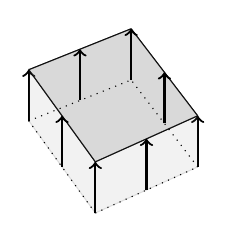
\begin{tikzpicture}[auto,scale = 0.65]
		\coordinate (A) at (0,0);
		\coordinate (B) at (2,0.9);
		\coordinate (C) at (-1.3,1.8);
		\coordinate (D) at (0.7,2.6);
		\coordinate (A') at (0,1);
		\coordinate (B') at (2,1.9);
		\coordinate (C') at (-1.3,2.8);
		\coordinate (D') at (0.7,3.6);
		\draw[->,thick] (B) -- (B');
		\draw (A') -- (B');
		\draw[->,thick] (C) -- (C');
		\draw (A') -- (C');
		\draw (B') -- (D');
		\draw (C') -- (D');
		\draw [fill = gray,draw = black,opacity = 0.1] (A) -- (B) -- (B') -- (A') -- (A);
		\draw [fill = gray,draw = black,opacity = 0.1] (A) -- (C) -- (C') -- (A') -- (A);
		\draw [fill = gray,draw = black,opacity = 0.3] (A') -- (B') -- (D') -- (C') -- (A');
		\draw[dotted](A) -- (B);
		\draw[dotted] (A) -- (C);
		\draw[dotted] (B) -- (D);
		\draw[dotted] (C) -- (D);
		\draw[->,thick] (D) -- (D');
		\draw[->,thick] (A) -- (A');
		\draw[->,thick] (-0.65,0.9) -- (-0.65,1.9);
		\draw[->,thick] (1,0.45) -- (1,1.45);
		\draw[->,thick] (-0.3,2.2) -- (-0.3,3.2);
		\draw[->,thick] (1.35,1.75) -- (1.35,2.75);
		\end{tikzpicture}
			\end{center}		
Observe that this is a directed dihomotopy but not a reversible dihomotopy since the dipaths followed by this dihomotopy (depicted by the arrows) are not reversible.
		
		
	\end{enumerate}

	%matchbox, croix suisse, segment dirig�
	
	
	

\section{Relation with the fundamental category}

\subsection{Classical case and direct extension}	
\label{subsec:funcla}

In classical algebraic topology, the fundamental groupoid of a topological space is an invariant of this space, in the following sense:

\begin{theo}[\cite{brown06}]
A homotopy equivalence $\map{f}{X}{Y}$ induces an equivalence of categories $\map{\pi_1(f)}{\pi_1(X)}{\pi_1(Y)}$.
\end{theo}

\begin{proof}
\label{theo:brown}
We prove the following first: a homotopy $H$ between $\map{f,g}{X}{Y}$ induces a natural transformation $\map{\sigma}{\pi_1(f)}{\pi_1(g)}$. Indeed, let $x$ be a point of $X$. $\sigma_x$ should be a homotopy class of paths from $f(x)$ to $g(x)$. We pose $\sigma_x = [H(x)]$. Let us prove that it is natural, that is, for every path $\pathto{\gamma}{x}{y}$, the two paths $(f\circ\gamma)\star H(y)$ and $H(x)\star(g\circ\gamma)$ from $f(x)$ to $g(y)$ are homotopic. Consider the homotopy $\map{H'}{[0,1]}{\pathspp{Y}{f(x)}{g(y)}}$ which maps $t \in [0,1]$ to the following path:
\begin{center}
\begin{tabular}{rc|lr}
 $s$ & $\mapsto$ & $H(x)(2s)$ & if $s \leq \frac{1-t}{2}$ \\
 & & $H(\gamma(2s+t-1))(1-t)$ & if $\frac{1-t}{2} \leq s \leq 1 - \frac{t}{2}$\\
  & & $H(y)(2s-1)$ & if $1 - \frac{t}{2} \leq s$
\end{tabular}
\end{center}
It is easy to check that $H'(0) = H(x)\star(g\circ\gamma)$ and $H'(1) = (f\circ\gamma)\star H(y)$.

Moreover, since the fundamental groupoid is a groupoid, any such natural transformation is automatically a natural isomorphism. Now, since $f\circ g$ and $g\circ f$ are both homotopic to identities then by the previous result, there are natural isomorphisms between $\pi_1(f)\circ\pi_1(g)$ and $\text{id}_{\pi_1(Y)}$, and between $\pi_1(g)\circ\pi_1(f)$ and $\text{id}_{\pi_1(X)}$.
\end{proof}

Let us try to do the same in $\dtop$. First:

\begin{lemme}[\cite{grandis09}]
\label{lemme:diheqnat}
Let $I \in \{\dirseg,\revseg\}$. Then a $I$-dihomotopy between $f$ and $g$ induces a natural transformation from $\funcat{f}$ to $\funcat{g}$. If $I = \revseg$, then this natural transformation is an isomorphism.
\end{lemme}

\begin{proof}
We do exactly the same proof. Observe that $\sigma_x$ is an isomorphism if $H(x)$ is a reversible dipath. The only thing to verify is that $H'$ is actually a dihomotopy, that is, it is with values in dipaths. Since dipaths are closed under concatenation and non-decreasing reparametrization, it is enough to prove that each piece is a dipath:
\begin{itemize}
	\item the first part is a non-decreasing reparametrization of $H(x)$ which is a dipath if $I \in \{\dirseg,\revseg\}$,
	\item idem for the third part,
	\item the second part is a non-decreasing reparametrization of $s \mapsto H(\gamma(s))(1-t)$ with $t$ fixed. Since $x \mapsto H(x)(1-t)$ is a dimap and $\gamma$ is a dipath, then $s \mapsto H(\gamma(s))(1-t)$ is a dipath.
\end{itemize}
\end{proof}

\begin{coro}[\cite{grandis09}]
\label{coro:revfun}
If $f$ is a reversible equivalence, then $\funcat{f}$ is a equivalence of categories. This result is false for undirected and directed equivalences.
\end{coro}

A counter-example for the other cases is the directed segment: we have seen that it is (un)directedly equivalent to a point. Since, the fundamental category of $\dirseg$ is isomorphic to the poset $([0,1], \leq)$ (and so is not a groupoid), it cannot be equivalent to the fundamental category of a point (which is a groupoid). This result implies in particular that the matchbox cannot be reversibly equivalent to a point since its fundamental category is not a groupoid.






\subsection{Localization of a category}
\label{subsec:local}

In the previous subsection, we have seen that in the case of directed equivalences, the only problem is that there are too few isomorphisms in the fundamental category. So to turn the fundamental category into an invariant of directed equivalence, one should invert some of its morphisms. There is a general process of inverting morphisms in a category, which is called \textbf{localization} \cite{gabriel67}.

We start with a category $\C$ and a subclass $W$ of morphisms of $\C$. A \textbf{localization of $\C$ at $W$} is a category $\loca{\C}{W}$ together with a functor $\map{Q_{\C,W}}{\C}{\loca{\C}{W}}$ such that:
\begin{itemize}
	\item for every $w \in W$, $Q_{\C,W}(w)$ is an isomorphism,
	\item for every functor $\map{F}{\C}{\D}$ such that for every $w \in W$, $F(w)$ is a isomorphism, there is a unique functor $\map{\tilde{F}}{\loca{\C}{W}}{\D}$ such that $F = \tilde{F}\circ Q_{\C,W}$.
\end{itemize}
As usual, the localization is unique up to isomorphism, when it exists. For the existence, there is a general construction for localizations. We need first some usual constructions from category theory.

Given a class $O$ and for every pair $c,c' \in \mathcal{O}$, a set $M_{c,c'}$, the \textbf{free category $(O,M)^\star$ generated by $O, M$} is the (possibly large) category whose:
\begin{itemize}
	\item objects are the elements of $O$,
	\item the morphisms from $c$ to $c'$ are finite non-empty sequences $(c ; f_1, \ldots, f_n ; c')$ such that there are $c_0$, $c_1$, \ldots, $c_n$ with $c_0 = c$, $c_n = c'$, and for every $i$, $f_i \in M_{c_{i-1},c_i}$,
	\item the composition is the concatenation, $$(c'; g_1, \ldots, g_p ; c'')\circ(c;f_1, \ldots, f_n;c') = (c;f_1, \ldots, f_n, g_1, \ldots, g_p;c''),$$
	\item identity of $c$ is $(c; \, ; c)$.
\end{itemize}


\noindent A \textbf{congruence} $R$ on a (possibly large) category $\C$ is a collection $(R_{c,c'})_{c,c' \in \ob{\C}}$, where $R_{c,c'}$ is an equivalence relation on $\C(c,c')$ such that:
\begin{itemize}
	\item for every $\map{f,f'}{c}{c'}$, for every $\map{g}{c''}{c}$, if $(f,f') \in R_{c,c'}$ then $(f\circ g,f'\circ g) \in R_{c'',c'}$,
	\item for every $\map{f,f'}{c}{c'}$, for every $\map{g}{c'}{c''}$, if $(f,f') \in R_{c,c'}$ then $(g\circ f,g\circ f') \in R_{c,c''}$.
\end{itemize}
Given a collection of relations $\sim \,= (\sim_{c,c'})$, there always is a smallest congruence (for inclusion) such that for every $c, c'$, $\sim_{c,c'} \,\subseteq R_{c,c'}$. It is called the \textbf{congruence generated by $\sim$}.
The \textbf{quotient} of a (possibly large) category $\C$ by a congruence $R$, is the (possibly large) category $\C/R$ whose:
\begin{itemize}
	\item objects are objects of $\C$,
	\item morphisms from $c$ to $c'$ are elements of $\C(c,c')/R_{c,c'}$, those elements are written $[f]_R$,
	\item identity of $c$ is $[id_c]_R$,
	\item composition is given by $[f]_R\circ[g]_R = [f\circ g]_R$ (which is well defined by definition of a congruence).
\end{itemize}

Let us come back to the localization of $\C$ at $W$. We consider $O = \ob{\C}$ and $M_{c,c'} = \C(c,c')\sqcup\{\bar{f} \mid \map{f}{c'}{c} \in W\}$. Let $R$ be the congruence on $(O,M)^\star$ generated by the following relations:
\begin{itemize}
	\item $(c;id_c;c) \sim (c; \, ; c)$,
	\item $(c; f, g;c') \sim (c;g\circ f;c')$,
	\item $(c; f,\bar{f};c) \sim (c; \, ; c)$,
	\item $(c;\bar{f},f;c) \sim (c; \, ;c)$.
\end{itemize}

\begin{theo}[\cite{gabriel67}]
When $(O,M)^\star/R$ is a category (i.e., not large), then it is the localization of $\C$ at $W$. In particular, when $\C$ is small, then $\loca{\C}{W}$ exists and is small.
\end{theo}

\begin{proof}
There is a functor $\map{Q}{\C}{(O,M)^\star/R}$ which maps:
\begin{itemize}
	\item every object $c$ to $c$,
	\item every morphism $\map{f}{c}{c'}$ to $[(c;f;c')]_R$.
\end{itemize}
$$Q(id_c) = [(c;id_c;c)]_R = [(c;\,;c)]_R = [id_c]_R = id_c$$
$$Q(g\circ f) = [(c;g\circ f;c'')]_R = [(c;f,g;c'')]_R = [(c';g;c'')\circ(c;f;c')]_R = [(c';g;c'')]_R\circ[(c;f;c')]_R = Q(g)\circ Q(f)$$
Given a morphism $w \in W$, $Q(w) = [(c;w;c')]_R$. Let us prove that $[(c';\bar{w};c)]_R$ is an inverse of $Q(w)$:
$$Q(w)\circ[(c';\bar{w};c)]_R = [(c;w;c')]_R\circ[(c';\bar{w};c)]_R = [(c;w;c')\circ(c';\bar{w};c)]_R = [(c';\bar{w},w;c')]_R = [(c'; ;c')]_R = id_{c'}$$
Given another such functor $\map{F}{\C}{\D}$. Define $\map{\tilde{F}}{(O,M)^\star/R}{\D}$ to be the functor which maps:
\begin{itemize}
	\item every object $c$ to $F(c)$,
	\item every morphism $[(c;h_1,\ldots, h_n;c')]_R$ to $h'_n\circ\ldots\circ h'_1$ where $h'_i$ is equal to $F(h_i)$ if $h_i$ is a morphism of $\C$, otherwise $h_i = \bar{f_i}$ and $h'_i$ is equal $F(f_i)^{-1}$.
\end{itemize}
It is well-defined:
$$\tilde{F}([(c;id_c;c)]_R) = id_{F(c)} = \tilde{F}([(c;\,;c)]_R)$$
$$\tilde{F}([(c;f,g;c')]_R) = F(g)\circ F(f) = F(g\circ f) = \tilde{F}([(c;g\circ f;c')]_R)$$
$$\tilde{F}([(c; f,\bar{f};c)]_R) = F(f)^{-1}\circ F(f) = id_{F(c)} = \tilde{F}([(c; \, ; c)]_R)$$
It is easy to check that it is a functor, that $F = \tilde{F}\circ Q$ and it is the only such functor.
\end{proof}
	
Let us note $\catpair$ be the category whose objects are pairs $(\C,W)$ of a small category $\C$ and of a subset $W$ of morphisms of $\C$ and whose morphisms from $(\C,W)$ to $(\C',W')$ are functors $\map{F}{\C}{\C'}$ such that for every $f \in W$, $F(f) \in W'$. The localization extends to a functor $\map{\Lambda}{\catpair}{\cat}$: for a morphism $\map{F}{(\C,W)}{(\C',W')}$, the functor $Q_{\C',W'}\circ F$ from $\C$ to $\loca{\C'}{W'}$ maps every elements of $W$ to an isomorphism. So there is a unique functor $\map{\Lambda(F)}{\loca{\C}{W}}{\loca{\C'}{W'}}$ such that $\Lambda(F)\circ Q_{\C,W} = Q_{\C',W'}\circ F$. Actually, it even extends to a strict 2-functor:

\begin{prop}
\label{prop:grpnat}
Let $\map{F,G}{(\C,W)}{(\C',W')}$ be functors in $\catpair$. If there is a natural transformation $\map{\sigma}{F}{G}$ then there is natural transformation $\map{\Lambda(\sigma)}{\Lambda(F)}{\Lambda(G)}$.
%\dessin
\end{prop}

\begin{proof}
We define $\Lambda(\sigma)_c$ as $[(F(c); \sigma_c; G(c))]$. To prove the naturality it is enough to prove the following two commutativity conditions:
\begin{itemize}
	\item given a morphism $\map{f}{c}{c'}$ of $\C$:\\
	\begin{center}
		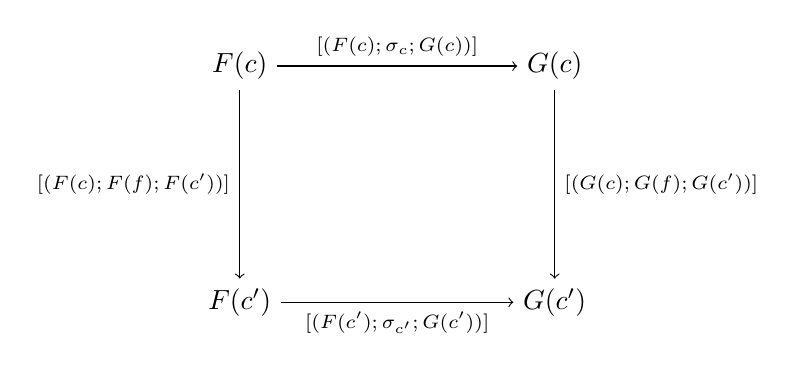
\begin{tikzpicture}[scale=1]
		
	\node (fcp) at (0,0) {$F(c')$};
	\node (gcp) at (4,0) {$G(c')$};
	\node (fc) at (0,3) {$F(c)$};
	\node (gc) at (4,3) {$G(c)$};
	
	\path[->,font=\scriptsize]
		(fc) edge node[above]{$[(F(c);\sigma_c;G(c))]$} (gc)
		(fcp) edge node[below]{$[(F(c');\sigma_{c'};G(c'))]$} (gcp)
		(fc) edge node[left]{$[(F(c);F(f);F(c'))]$} (fcp)
		(gc) edge node[right]{$[(G(c);G(f);G(c'))]$} (gcp);
			
\end{tikzpicture}
	\end{center}
	which is true since:
	\begin{center}
		\begin{tabular}{rcl}
		 $[(G(c);G(f);G(c'))]\circ[(F(c);\sigma_c;H(c))]$ & $=$ & $[(F(c);G(f)\circ\sigma_c;G(c'))]$\\
		 & $=$ & $[(F(c);\sigma_{c'}\circ F(f);G(c'))]$\\
		  & $=$ & $[(F(c');\sigma_{c'};G(c'))]\circ[(F(c);F(f);F(c'))]$
		\end{tabular}
	\end{center}
	\item given a morphism $\map{f}{c}{c'} \in W$:\\
	\begin{center}
		\begin{tikzpicture}[scale=1]
		
	\node (fcp) at (0,0) {$F(c')$};
	\node (gcp) at (4,0) {$G(c')$};
	\node (fc) at (0,3) {$F(c)$};
	\node (gc) at (4,3) {$G(c)$};
	
	\path[->,font=\scriptsize]
		(fc) edge node[above]{$[(F(c);\sigma_c;G(c))]$} (gc)
		(fcp) edge node[below]{$[(F(c');\sigma_{c'};G(c'))]$} (gcp)
		(fcp) edge node[left]{$[(F(c);F(f);F(c'))]^{-1} = \Lambda(F)([(c';\bar{f};c)])$} (fc)
		(gcp) edge node[right]{$\Lambda(G)([(c';\bar{f};c)]) = [(G(c);G(f);G(c'))]^{-1}$} (gc);
			
\end{tikzpicture}
	\end{center}
	which is true since $\Lambda(F)([c';\bar{f};c)]) = [(F(c);F(f);F(c')]^{-1}$, idem for $G$ and since $\sigma$ is natural $\sigma_{c'}\circ F(f) = G(f)\circ\sigma_{c}$, so $[(F(c);\sigma_{c'}\circ F(f);G(c'))] = [(F(c);G(f)\circ\sigma_{c};G(c'))]$, that is, $[(G(c);G(f);G(c'))]^{-1}\circ[(F(c');\sigma_{c'};G(c'))] = [(F(c);\sigma_{c};G(c))]\circ[(F(c);F(f);F(c'))]^{-1}$.
\end{itemize}
\end{proof}




\subsection{Groupoidification}
\label{subsec:grpi}

We have seen that directed equivalences do not induce equivalences of fundamental categories. The main problem was that there were too few isomorphisms. Here, we tackle this problem by inverting morphisms of the fundamental category using localization. But since we have no information on which morphisms are needed to be inverted, we will invert all the morphisms. This process is called \textbf{groupoidification}.

There is a functor $\map{\kappa}{\cat}{\catpair}$ which maps every category $\C$ to the pair $(\C,\text{Mor}(\C))$. The groupoidification functor is the composition $\map{\Lambda\circ\kappa}{\cat}{\cat}$. Let us denote by $Gp$ this functor. Actually, $Gp$ is with values in groupoids, and even more, this groupoid is universal in the following sense:

\begin{prop}
For every small category $\C$, $Gp(\C)$ is a small groupoid such that for every functor $\map{F}{\C}{\D}$ where $\D$ is a groupoid, then there is a unique functor $\map{\tilde{F}}{Gp(\C)}{\D}$ such that $F = \tilde{F} \circ Q_{\C,\text{Mor}(\C)}$.
\end{prop}

\begin{proof}
It is a groupoid since every morphism of $Gp(\C)$ is of the form $[(c;f_1,\ldots, f_n;c')]$ with either $f_i$ a morphism of $\C$, either $f_i = \bar{g_i}$ for some morphism $g_i$ of $\C$ and so the inverse of such a morphism is $[(c';h_n, \ldots, h_1;c)]$ with $h_i = \bar{f_i}$ if $f_i$ is a morphism of $\C$, $h_i = g_i$ if $f_i = \bar{g_i}$.

The universal property is a particular case of the universal property of a localization.
\end{proof}

From this study, we can prove what we were looking for:

\begin{theo}
If $\map{f}{X}{Y}$ is a directed equivalence, then $\map{Gp(\funcat{f})}{Gp(\funcat{X})}{Gp(\funcat{Y})}$ is an equivalence of categories.
\end{theo}

\begin{proof}
We have seen in Lemma \ref{lemme:diheqnat} that a directed homotopy between $f$ and $g$ induces a natural transformation from $\funcat{f}$ to $\funcat{g}$. Then from Proposition \ref{prop:grpnat}, a directed homotopy induces a natural transformation from $Gp(\funcat{f})$ to $Gp(\funcat{g})$. Since the groupoidification is a groupoid, this natural transformation is automatically a natural isomorphism.
\end{proof}

Moreover, inducing an equivalence between groupoidifications is weaker than inducing an equivalence:

\begin{prop}
\label{lem:locaequi}
Let $\map{F}{(\C,W)}{(\C',W')}$ and $\map{G}{(\C',W')}{(\C,W)}$ be such that $F$ and $G$ form an equivalence of categories. Then $\tilde{F}$ and $\tilde{G}$ form an equivalence between $\loca{\C}{W}$ and $\loca{\C'}{W'}$.
\end{prop}

In particular, since a functor $\map{F}{\C}{\C'}$ is automatically a morphism $\map{F}{(\C,\text{Mor}(\C))}{(\C',\text{Mor}(\C'))}$, an equivalence of categories induces an equivalence between the groupoidifications.

\begin{proof}
First notice that given two functors $\map{F,G}{(\C,W)}{(\C',W')}$ and a natural transformation $\map{\sigma}{F}{G}$ then $\map{\tilde{\sigma}}{\tilde{F}}{\tilde{G}}$ defined as $\tilde{\sigma}_c = [(F(c);\sigma_c;G(c))]$ is also natural. Consequently, if $\sigma$ is a natural isomorphism, i.e., $\sigma_c$ is an isomorphism for all $c$, then $\tilde{\sigma}_c$ is also an isomorphism for all $c$.
\end{proof}






\section{Inessential morphisms and the category of components}
\label{sec:inecomp}

\subsection{Yoneda morphisms, inessential morphisms}
\label{subsec:inemor}

One problem of the groupoidification is that we completely loose non-cancellative behaviors, since a groupoid is left and right cancellative. This implies for example that the functor $Q_{\C,W}$ is not faithful when $\C$ is not cancellative, which is the case for the fundamental category of the matchbox. The real problem comes from the fact that, in the groupoidification, we invert everything, in particular things that do not behave like isomorphisms. For example, for the non-cancellative behaviors, we have morphisms such that $h\circ f = h\circ g$ and $f\neq g$, and so $h$ is far from being an isomorphism. 

The idea from \cite{goubault07} is to localize at some set of morphisms that behave like isomorphisms. We do the same here, except that the axioms defining those morphisms are slightly different.

We say that a morphism $\map{f}{c}{c'}$ is a \textbf{Yoneda morphism} if:
\begin{itemize}
	\item \textbf{right cancellation:} for every object $c''$ such that $\C(c',c'') \neq \varnothing$, the function
	$$c''\circ f : \C(c',c'') \rightarrow \C(c,c'') ~~~ g \mapsto g \circ f$$
	is a bijection.
	\item \textbf{left cancellation:} for every object $c''$ such that $\C(c'',c) \neq \varnothing$, the function
	$$f\circ c'' : \C(c'',c) \rightarrow \C(c'',c') ~~~ g \mapsto f \circ g$$
	is a bijection.
\end{itemize}

For example, the morphism $h$ from non-cancellation is not a Yoneda morphism. In particular, the dihomotopy class of the red dipath in the matchbox from picture \ref{fig:matchdihom} is not a Yoneda morphism in $\funcat{\matchbox}$.

Another convenient property of the class of isomorphisms is the following. We say that a subclass $W$ of morphisms has:
\begin{itemize}
	\item \textbf{right Ore condition:} for every $\map{f}{c}{c'} \in W$, for every $\map{g}{c''}{c'}$, there are $\map{f'}{d}{c''} \in W$ and $\map{g'}{d}{c} \in \C$ for some $d$ such that $f\circ g' = g\circ f'$
	\begin{center}
	\begin{tikzpicture}[scale=2]
		\node (A) at (0,1) {$d$};
		\node (B) at (1.2,1) {$c$};
		\node (C) at (0,0) {$c''$};
		\node (D) at (1.2,0) {$c'$};
		\path[->,font=\scriptsize,dotted]
		(A) edge node[above]{$g'\in\C$} (B)
		(A) edge node[left]{$f'\in W$} (C);
		\path[->,font=\scriptsize]
		(C) edge node[below]{$g\in\C$} (D)
		(B) edge node[right]{$f\in W$} (D);
	\end{tikzpicture}
	\end{center}
	\item \textbf{left Ore condition:} for every $\map{f}{c}{c'} \in W$ and every $\map{g}{c}{c''} \in \C$ there are $\map{f'}{c''}{d} \in W$ and $\map{g'}{c'}{d} \in \C$ for some $d$ such that $f'\circ g = g'\circ f$.
	\begin{center}
	\begin{tikzpicture}[scale=2]
		\node (A) at (0,1) {$c$};
		\node (B) at (1.2,1) {$c''$};
		\node (C) at (0,0) {$c'$};
		\node (D) at (1.2,0) {$d$};
		\path[->,font=\scriptsize]
		(A) edge node[above]{$g\in\C$} (B)
		(A) edge node[left]{$f\in W$} (C);
		\path[->,font=\scriptsize,dotted]
		(C) edge node[below]{$g'\in\C$} (D)
		(B) edge node[right]{$f'\in W$} (D);
	\end{tikzpicture}
	\end{center}
\end{itemize}

Those axioms are strengthened in \cite{goubault07} where they require closure under pullbacks and pushouts instead. Those properties are important in our study for the following reason. Let us come back to the Swiss flag d-space from Section \ref{subsec:exa}. Consider the dipath whose image is depicted in red below:
			\begin{center}
				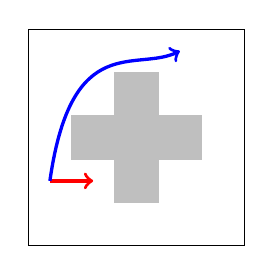
\begin{tikzpicture}[auto,scale = 0.55]
\draw (0,0) rectangle (5,5);
\draw [fill = gray!50,draw = gray!50] (1,2) rectangle (4,3);
\draw [fill = gray!50,draw = gray!50] (2,1) rectangle (3,4);
\draw[->,red,very thick] (0.5,1.5) -- (1.5,1.5);
\draw[->, blue, very thick] (0.5,1.5) .. controls (1,5) and (2.5,4) .. (3.5,4.5);
\end{tikzpicture}
			\end{center}	
\noindent It is easy to check that the dihomotopy class of this dipath is a Yoneda morphism in $\funcat{SF}$. However, this dipath leads to an unsecured region, that is, a set of states that can only lead to a deadlock. Inverting this morphism is no good, since it will identify unsecured states with secured states. That is why the right Ore condition is interesting: this dipath fails this condition with the dipath depicted in blue, there is no way to complete the square with dipaths. Symmetrically, the left Ore condition avoids the identification of inaccessible states with accessible ones.



%\textcolor{red}{Develop the example of the Swiss cross to explain why it is important}\\

\begin{defi}
Given a small category $\C$, we define a \textbf{Yoneda system $\Theta$} of morphisms of $\C$ as a subset of morphisms of $\C$ such that:
\begin{itemize}
	\item every element of $\Theta$ is left and right cancellative,
	\item $\Theta$ has left and right Ore conditions.
\end{itemize}
\end{defi}


\begin{lemme}
The set of Yoneda systems of morphisms of $\C$ is a non-empty complete lattice for inclusion.
\end{lemme}

\begin{proof}
The set of Yoneda systems is non-empty since the set of isomorphisms is a Yoneda system. The $\sup$ is given by the union.
\end{proof}

\begin{defi}
We denote by $\ine{\C}$ the maximal Yoneda system of morphisms of $\C$. We call its elements \textbf{inessential morphisms of $\C$}.
\end{defi}

For example, for the d-space SF, the inessential morphisms of $\funcat{SF}$ are the dihomotopy classes of dipaths that are included in the zones delimited by dotted lines (modulo boundary conditions) here:
			\begin{center}
				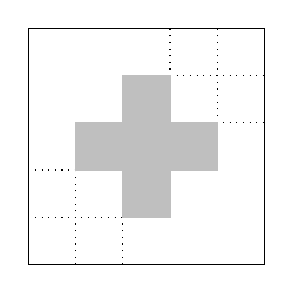
\begin{tikzpicture}[auto,scale = 0.6]
\draw (0,0) rectangle (5,5);
\draw [dotted] (1,0) -- (1,2);
\draw[dotted] (2,0) -- (2,2);
\draw[dotted] (0,1) -- (2,1);
\draw[dotted] (0,2) -- (2,2);
\draw [dotted] (3,3) -- (3,5);
\draw[dotted] (4,3) -- (4,5);
\draw[dotted] (3,3) -- (5,3);
\draw[dotted] (3,4) -- (5,4);
\draw [fill = gray!50,draw = gray!50] (1,2) rectangle (4,3);
\draw [fill = gray!50,draw = gray!50] (2,1) rectangle (3,4);
\end{tikzpicture}
			\end{center}	


\begin{lemme}
$\ine{\C}$ makes $\C$ into a category with weak equivalences, i.e., $\ine{\C}$ is a subcategory of $\C$ which contains the isomorphisms and which has the 2-out-of-3 property. Moreover, $\ine{\C}$ has the 2-out-of-6 property.
\end{lemme}

\begin{proof}~
\begin{itemize}
	\item \textbf{contains isomorphisms:} the set of isomorphisms is a Yoneda system.
	\item \textbf{$\ine{\C}$ is closed under composition:} let $\Theta$ be a Yoneda system. Let $\langle\Theta\rangle$ be the set $$\{f_1\circ\ldots\circ f_n \mid n \geq 1, f_i \in \Theta\}.$$
	$\langle\Theta\rangle$ is closed under composition. It is enough to prove that $\langle\Theta\rangle$ is a Yoneda system:
		\begin{itemize}
			\item \textbf{left, right cancellation:} left and right cancellative morphisms are closed under composition,
			\item \textbf{left, right Ore condition:} by induction on $n$:
			
	\begin{center}
			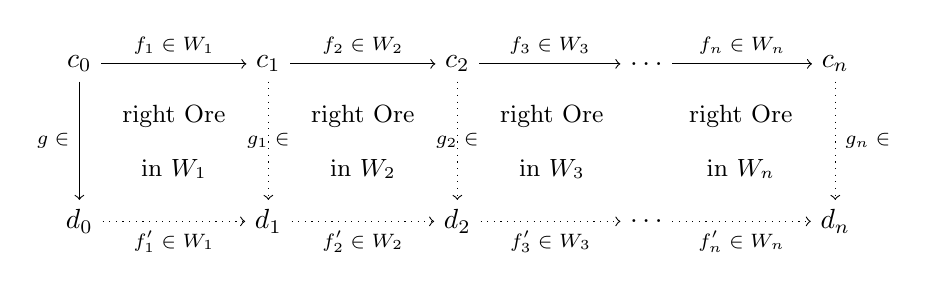
\begin{tikzpicture}[scale=2]
		\node (A) at (0,1) {$c_0$};
		\node (B) at (1.2,1) {$c_1$};
		\node (C) at (0,0) {$d_0$};
		\node (D) at (1.2,0) {$d_1$};
		\node (E) at (2.4,1) {$c_2$};
		\node (F) at (2.4,0) {$d_2$};
		\node (G) at (3.6,1) {$\ldots$};
		\node (H) at (3.6,0) {$\ldots$};
		\node (I) at (4.8,1) {$c_n$};
		\node (J) at (4.8,0) {$d_n$};
		\node (K1) at (0.6,0.666667) {\small{right Ore}};
		\node (K2) at (0.6,0.333333) {\small{in $W_1$}};
		\node (L1) at (1.8,0.666667) {\small{right Ore}};
		\node (L2) at (1.8,0.333333) {\small{in $W_2$}};
		\node (M1) at (3,0.666667) {\small{right Ore}};
		\node (M2) at (3,0.333333) {\small{in $W_3$}};
		\node (N1) at (4.2,0.666667) {\small{right Ore}};
		\node (N2) at (4.2,0.333333) {\small{in $W_n$}};
		\path[->,font=\scriptsize]
		(A) edge node[above]{$f_1\in W_1$} (B)
		(A) edge node[left]{$g\in\C$} (C)
		(B) edge node[above]{$f_2 \in W_2$} (E)
		(E) edge node[above]{$f_3 \in W_3$} (G)
		(G) edge node[above]{$f_n \in W_n$} (I) ;
		\path[->,font=\scriptsize,dotted]
		(C) edge node[below]{$f'_1\in W_1$} (D)
		(B) edge node{$g_1\in\C$} (D)
		(D) edge node[below]{$f'_2 \in W_2$} (F)
		(E) edge node{$g_2 \in \C$} (F)
		(F) edge  node[below]{$f'_3 \in W_3$} (H)
		(H) edge node[below]{$f'_n \in W_n$} (J)
		(I) edge node[right]{$g_n \in \C$} (J);
	\end{tikzpicture}
	\end{center}	
			
		\end{itemize}
	\item \textbf{2-out-of-3 property:} let $\Theta$ be a Yoneda system. Let $\lceil\Theta\rceil$ be the set $$\{f \mid \exists g,h \in \Theta, \, g = f\circ h\}\cup\{f \mid \exists g,h \in \Theta, \, g = h\circ f\}\cup\Theta.$$
	We prove that $\lceil\Theta\rceil$ is a Yoneda system:
		\begin{itemize}
			\item \textbf{left, right cancellation:} let $\map{f}{a}{b}$ be such that there exist $\map{g}{b}{c} \in \Theta$ and $\map{h}{a}{c} \in \Theta$ such that $h = g\circ f$, the other case is symmetric. The left cancellation is easy, since if $\C(d,a) \neq \varnothing$, the function $f\circ d$ is equal to $(g\circ d)^{-1}\circ(h\circ d)$ which is a bijection. For the right cancellation, let $d$ with $\C(b,d) \neq \varnothing$. By the left Ore condition, there is a morphism $\map{k}{d}{e} \in \Theta$ with $\C(c,e) \neq \varnothing$. Let us prove that $d\circ f$ is injective and surjective.
				\begin{itemize}
					\item \textbf{injective:} let $\map{\alpha_1,\alpha_2}{b}{d}$ be such that $\alpha_1\circ f = \alpha_2\circ f$. So $k\circ\alpha_1\circ f = k \circ \alpha_2\circ f$. Since $e\circ g$ is a bijection, there are $\map{\beta_1, \beta_2}{c}{e}$ such that $k\circ\alpha_i = \beta_i\circ g$. So $\beta_i\circ h = \beta_i\circ g\circ f = k\circ\alpha_i\circ f$ and since $e\circ h$ is a bijection, $\beta_1 = \beta_2$, thus $k \circ \alpha_1 = k \circ\alpha_2$. Since $k\circ b$ is a bijection, $\alpha_1 = \alpha_2$.
					\item \textbf{surjective:} let $\map{\alpha}{a}{d}$, so $\map{k\circ\alpha}{a}{e}$. Since $e\circ h$ is a bijection, there is $\map{\beta}{c}{e}$ such that $k\circ\alpha = \beta\circ h = \beta\circ g \circ f$. Since $k\circ b$ is a bijection, there is $\map{\gamma}{b}{d}$ such that $k\circ\gamma = \beta\circ g$. Since $k\circ\alpha = k\circ\gamma\circ f$ and $k\circ a$ is a bijection, $\alpha = \gamma\circ f$.
				\end{itemize}
			\item \textbf{left, right Ore condition:} let $\map{f}{a}{b}$ be such that there exist $\map{g}{b}{c} \in \Theta$ and $\map{h}{a}{c} \in \Theta$ such that $h = g\circ f$, the other case is symmetric.
				\begin{itemize}
					\item \textbf{right:} let $\map{\alpha}{d}{b}$. By the right Ore condition on $h$ and $g\circ\alpha$, there $\map{\beta}{e}{d} \in \Theta$ and $\map{\gamma}{e}{a} \in \C$ such that $g\circ\alpha\circ\beta = h\circ\gamma = g\circ f\circ\gamma$. Since $g\circ e$ is a bijection, $\alpha\circ\beta = f\circ\gamma$.
					\item \textbf{left:} let $\map{\alpha}{a}{d}$. By the left Ore condition on $h$ and $\alpha$, there are $\map{\beta}{d}{e} \in \Theta$ and $\map{\gamma}{c}{e} \in \C$ such that $\beta\circ\alpha = \gamma\circ h = (\gamma\circ g)\circ f$.
				\end{itemize}
		\end{itemize}
		Now define $X_0 = \Theta$, $X_{2i+1} = \langle X_{2i} \rangle$ and $X_{2i+2} = \lceil X_{2i+1} \rceil$. Let $X_\infty = \bigcup\limits_{i\in\nat} X_i$. By what we just proved, for every $i$, $X_i$ is a Yoneda system which contains $\Theta$, so $X_\infty$ is a Yoneda system which contains $\Theta$. Moreover, $X_\infty$ has the 2-out-of-3 property.
		\item \textbf{2-out-of-6 property:} Let $\Theta$ be a Yoneda system. Let $\map{u}{a}{b}$, $\map{v}{b}{c}$ and $\map{w}{c}{d}$ be such that $v\circ u$ and $w\circ v \in \Theta$. It is enough to prove that $\Theta\cup\{v\}$ is a Yoneda. Indeed, if $\Theta = \ine{\C}$, then this prove that $v \in \ine{\C}$ by maximality. Since $\ine{\C}$ has the 2-out-of-3 property, this prove that $u$ and $w$ are also in $\ine{\C}$. Since $\ine{\C}$ is closed under composition, this prove that $w\circ v\circ u \in \ine{\C}$.
			\begin{itemize}
				\item \textbf{left, right cancellation:} let us do the right cancellation, the left is symmetric. Let $e$ such that $\C(c,e) \neq \varnothing$. Let us prove that $\map{e\circ v}{\C(c,e)}{\C(b,e)}$ is injective and bijective.
					\begin{itemize}
						\item \textbf{injective:} let $\map{\alpha_1,\alpha_2}{c}{e}$ be such that $\alpha_1\circ v = \alpha_2\circ v$. So $\alpha_1 \circ v \circ u = \alpha_2 \circ v\circ u$ and since $e\circ(v\circ u)$ is a bijection, $\alpha_1 = \alpha_2$.
						\item \textbf{surjective:} let $\map{\alpha}{b}{e}$. Since $e\circ(v\circ u)$ is a bijection, there is $\map{\beta}{c}{e}$ such that $\alpha\circ u = \beta\circ v\circ u$. To prove surjectivity, it is then enough to prove that $e\circ u$ is injective.
						\item \textbf{$e\circ u$ is injective:} let $\map{\alpha_1,\alpha_2}{b}{e}$ be such that $\alpha_1\circ u = \alpha_2 \circ u$. Since $\C(b,e) \neq \varnothing$, then by the left Ore condition on $w\circ v \in \Theta$, there is $\map{\beta}{e}{f} \in \Theta$ such that $\C(d,f) \neq \varnothing$. So $\beta\circ\alpha_1\circ u = \beta\circ\alpha_2\circ u$. Since $f\circ(w\circ v)$ is a bijection, there is $\map{\gamma_1,\gamma_2}{d}{f}$ such that $\gamma_i\circ w\circ v = \beta\circ\alpha_i$. Thus $\gamma_1\circ w\circ v \circ u = \gamma_2\circ w \circ v \circ u$. Since $f\circ(v\circ u)$ is a bijection, $\gamma_1\circ w = \gamma_2\circ w$ and thus $\beta\circ\alpha_1 = \beta\circ\alpha_2$. Since $\beta\circ b$ is a bijection, $\alpha_1 = \alpha_2$.
					\end{itemize}
				\item \textbf{left, right Ore condition:} let us prove the right Ore condition, the other is symmetric. Let $\map{\alpha}{e}{c}$. By the right condition on $u\circ v \in \Theta$ and $\alpha$, there are $\map{\beta}{f}{e} \in \Theta$ and $\map{\gamma}{f}{a} \in \C$ such that $v \circ (u\circ\gamma) = \alpha\circ\beta$.
			\end{itemize}
\end{itemize}
\end{proof}


\begin{coro}
$\ine{\ine{\C}} = \ine{\C}$
\end{coro}

\begin{proof}
It is enough to prove that $\ine{\C}$ is a Yoneda system of $\ine{\C}$:
\begin{itemize}
	\item \textbf{left, right cancellation:} we prove left cancellation. Let $\map{w}{a}{b} \in \ine{\C}$ and let $c$ besuch that $\ine{\C}(b,c) \neq \varnothing$. In particular, $\C(b,c) \neq \varnothing$ and $\map{c\circ w}{\C(b,c)}{\C(a,c)}$ is a bijection. It is enough to prove that:
		\begin{itemize}
			\item $c \circ w$ sends inessential morphisms to inessential morphisms: by closure under composition,
			\item $(c\circ w)^{-1}$ sends inessential morphisms to inessential morphisms: by the 2-out-of-3 property.
		\end{itemize}
	\item \textbf{left, right Ore condition:} we prove the left Ore condition. Let $\map{w}{a}{b}$ and $\map{w'}{a}{c}$ be inessential morphisms. By the left Ore condition in $\C$, there are a morphism $\map{\alpha}{b}{d} \in \C$ and an inessential morphism $\map{\beta}{c}{d}$ such that $\alpha\circ w = \beta\circ w'$. Then by the 2-out-of-3 property, $\alpha$ is also inessential.
\end{itemize}
\end{proof}





\subsection{Calculus of fractions and localizations}
\label{subsec:calfra}



The axioms of Yoneda systems are close to the axioms for having a \textbf{calculus of fractions} \cite{gabriel67}. These axioms are general conditions for the existence of the localization, regardless of the problems from set-theory. They also allow us to simplify the construction from section \ref{subsec:local}.

More concretely, given a category $\C$ and a subclass $W$ of morphisms, we say $W$ has a \textbf{calculus of right fractions} if:
\begin{itemize}
	\item $W$ is a subcategory of $\C$,
	\item $W$ has the right Ore condition,
	\item for every morphisms $\map{f,g}{a}{b} \in \C$ and $\map{h}{b}{c} \in W$ with $h\circ f = h\circ g$, then there is a morphism $\map{h'}{d}{a} \in W$ such that $f\circ h' = g\circ h$.
\end{itemize}
Dually, one can define what it means to say that $W$ has a calculus of left fractions. $\ine{\C}$ has then a calculus of right and left fractions since the last condition is implied by cancellation.

The main interest of a right calculus of fractions is that the construction of the localization $\loca{\C}{W}$ from Section \ref{subsec:local} can be simplified. Remember that morphisms were equivalence classes of sequences $f_1, \ldots, f_n$ where $f_i$ is either a morphism of $\C$, or a formal inverse of a morphism of $W$, i.e., those sequences are zig-zags of morphisms. By the right Ore condition and the closure under composition, those zig-zags are always equivalent to a span with one branch in $W$, and one branch in $\C$. More precisely, its objects are still those of $\C$, but this time, its morphisms from $a$ to $c$ are equivalence classes of spans $\spa{a}{w}{b}{f}{c}$ of morphisms of $\C$ with $\map{w}{a}{b} \in W$. We says that two spans $\spa{a}{w}{b}{f}{c}$ and $\spa{a'}{w'}{b'}{f'}{c'}$ are equivalent if there are morphisms $\map{s}{d}{b}$ and $\map{t}{d}{b'}$ such that $s \circ w = t\circ w' \in W$ and $s \circ f = t \circ f$. In particular, when $W$ has the 2-out-of-3 property, $s$ and $t$ are in $W$. We denote this equivalence class by $[\spa{a}{w}{b}{f}{c}]$. The composition $[\spa{a}{w}{b}{f}{c}]\circ[\spa{c}{w'}{d}{f'}{e}]$ is defined as follow: by the right Ore condition on $f$ and $w$, there are morphisms $w'' \in W$ and $f'' \in \C$ such that $f\circ w'' = w\circ f''$. The composition is then defined by $[\spa{a}{w\circ w''}{ }{f\circ f''}{e}]$. The dual construction can be made when $W$ has a calculus of left fractions. When $W$ has both calculus of left and right fractions, those two constructions coincide (up to isomorphism).

One other interest is that one can characterize when $W$ is \textbf{saturated}, i.e., when $W$ is exactly the set of morphisms which become isomorphisms through localization. More precisely, let $W' = \{f \mid Q_{\C,W}(f) \text{ is an iso}\}$. We say that $W$ is saturated when $W' = W$. In the case where $W$ has a calculus of fractions (either right or left), it is known \cite{borceux94} that $W$ is saturated if and only if $W$ has the 2-out-of-6 property. In particular, $\ine{\C}$ is saturated.



\subsection{The category of components}
\label{subsec:comcat}


Our goal now is to construct a localization of the fundamental category, mid-way between it and its groupoidification. We have seen that $\ine{\funcat{X}}$ has a calculus of right and left fractions and so its localization $\loca{\funcat{X}}{\ine{\funcat{X}}}$ is easy to compute. We denote this localization by $\comcat{X}$ and call it the \textbf{category of components}, following the denomination from \cite{goubault07}. More generally, given a small category $\C$, we denote by $\comcat{\C}$, the localization $\loca{\C}{\ine{\C}}$.

One should notice that this does not extend to a functor: indeed a dimap $\map{f}{X}{Y}$ induces a functor between category of components if it sends an element of $\ine{\funcat{X}}$ to an element of $\ine{\funcat{Y}}$, which is not the case in general. 

For example, since every isomorphism is inessential, the category of components of a groupoid is the groupoid itself. Another example is the fundamental category of the directed segment $\dirseg$. This category is isomorphic to the poset $([0,1], \leq)$ and so every morphism is inessential. So its category of components is its groupoidification. Let us denote by $\dicir$, the d-space whose underlying space is $S^1$, the circle, and whose dipaths are paths that turn anti-clockwise, that is, paths of the form $t \mapsto e^{i\Phi(t)}$ for some non-decreasing function $\map{\Phi}{[0,1]}{\RR}$. In this case, the only Yoneda morphisms of $\dicir$ are the identities, i.e., dihomotopy class of constant paths. Indeed, they are the only ones that induces bijections between Hom-sets by composition: if you take any non-constant dipath $\gamma$, say from $e^{i\theta}$ to $e^{i\theta'}$ then $\map{[\gamma]\circ\_}{\funcat{\dicir}(e^{i\theta'},e^{i\theta})}{\funcat{\dicir}(e^{i\theta},e^{i\theta})}$ is not surjective since it never reaches the class of the constant path. Hence $\comcat{\dicir} = \funcat{\dicir}$.

This time the functor $\map{R_\C = Q_{\C,\ine{\C}}}{\C}{\comcat{\C}}$ is faithful, and so we do not lose the non-cancellative behaviors. Indeed, let $\map{f,g}{c}{d}$ be such that $R_\C(f) = R_\C(g)$. $R_\C(f)$ is the equivalence class of the span $\spa{c}{\text{id}_c}{c}{f}{d}$ and this equality means that there are two morphisms $\map{s,t}{e}{c} \in \ine{\C}$ such that $s = t$ and $f\circ s = g\circ t$. Since $d\circ s$ is a bijection, $f = g$.





\subsection{Equivalence with a quotient}
\label{subsec:equiquo}

Another good property of this category of components is that, in concrete cases, it is equivalent to a generalized quotient of the fundamental category (which is not true in general for a localization). In \cite{goubault07}, the theory was introduced for loop-free categories, i.e., for categories whose endomorphisms and isomorphisms are identities (which is the case for the fundamental category of pospaces, or for geometric realization of SU/PV-programs). In the latter case, this allows one to compute a finite category which is equivalent to the category of components. See the tool ALCOOL \cite{alcool}.

For example, it is possible to prove that the category of components of the Swiss flag is equivalent to the category generated by the following directed graph:
	\begin{center}
		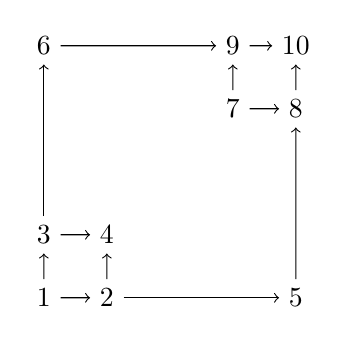
\begin{tikzpicture}[auto,scale = 0.8]
\node (1) at (0.5,0.5) {1};
\node (2) at (1.5,0.5) {2};
\node (3) at (0.5,1.5) {3};
\node (4) at (1.5,1.5) {4};
\node (5) at (4.5,0.5) {5};
\node (6) at (0.5,4.5) {6};
\node (7) at (3.5,3.5) {7};
\node (8) at (4.5,3.5) {8};
\node (9) at (3.5,4.5) {9};
\node (10) at (4.5,4.5) {10};
\node (com1) at (1,1) {$\circlearrowleft$};
\node (com1) at (4,4) {$\circlearrowleft$};
\draw [->] (1) to (3);
\draw [->] (1) to (2);
\draw [->] (3) to (4);
\draw [->] (2) to (4);
\draw [->] (2) to (5);
\draw [->] (3) to (6);
\draw [->] (7) to (9);
\draw [->] (7) to (8);
\draw [->] (9) to (10);
\draw [->] (8) to (10);
\draw [->] (5) to (8);
\draw [->] (6) to (9);
\end{tikzpicture}
	\end{center}
where $\circlearrowleft$ denotes a relation. Similarly, the category of components of the squared annulus is equivalent to the category generated by the following directed graph:
	\begin{center}
		\begin{tikzpicture}[auto,scale = 1.2]
\node (1) at (0.5,0.5) {1};
\node (2) at (2.5,0.5) {2};
\node (3) at (0.5,2.5) {3};
\node (4) at (2.5,2.5) {4};
\draw [->] (1) to (3);
\draw [->] (1) to (2);
\draw [->] (3) to (4);
\draw [->] (2) to (4);
\end{tikzpicture}
	\end{center}
In particular, these categories are not equivalent.

Actually, this phenomenon is more general, but the quotient used is trickier. Let us start by recalling the construction of a generalized quotient from \cite{bednarczyk99}. A \textbf{generalized congruence} on a small category $\C$ is the following data:
\begin{itemize}
	\item an equivalence relation $\simeq_o$ on objects of $\C$,
	\item a partial equivalence relation (i.e., symmetric and transitive relation) $\simeq_m$ on $Mor_+(\C)$ (i.e., the set of non-empty finite sequences of morphisms of $\C$). We call the set $\{\gamma\in Mor_+(\C) \mid \gamma \simeq \gamma\}$ the \textbf{support of $\simeq_m$}.
\end{itemize}
These data must satisfy:
\begin{itemize}
	\item if $(\beta_m, \ldots, \beta_0,\alpha_n, \ldots, \alpha_0)$ is in the support of $\simeq_m$, then source of $\beta_0 \simeq_o$ target of $\alpha_n$,
	\item if $(\beta_m,\ldots, \beta_0) \simeq_m (\alpha_n,\ldots,\alpha_0)$, then target of $\beta_m \simeq_o$ target of $\alpha_n$,
	\item if $c \simeq_o d$, then $(id_c) \simeq_m (id_d)$,
	\item if $(\beta_m,\ldots, \beta_0) \simeq_m (\alpha_n,\ldots,\alpha_0)$, 
$(\gamma_p,\ldots,\gamma_0) \simeq_m (\delta_q,$ $\ldots,\delta_0)$ and source of $\beta_0 \simeq_o$ target of $\alpha_n$, then $$(\beta_m,\ldots, \beta_0,\alpha_n,\ldots,\alpha_0) \simeq_m (\gamma_p,\ldots,\gamma_0,\delta_q,\ldots,\delta_0),$$
	\item if $\alpha$ and $\beta$ are composable (i.e., source of $\beta$ = target of $\alpha$), then $(\beta,\alpha) \simeq_m (\beta\circ\alpha)$.
\end{itemize}
Given a relation $R_0$ on objects of $\C$ and a relation $R_m$ on $Mor_+(\C)$, there is a smallest (for inclusion) generalized congruence that contains $(R_0,R_m)$ \cite{bednarczyk99}.\\
Given a generalized congruence $(\simeq_o,\simeq_m)$ on $\C$, we define the \textbf{generalized quotient $\C/(\simeq_o,\simeq_m)$} as the category whose:
\begin{itemize}
	\item objects are equivalence classes $[x]_0$ of objects of $\C$ modulo $\simeq_o$,
	\item morphisms from $[x]_0$ to $[y]_0$ are equivalence classes 
$$[(\alpha_n,\ldots,\alpha_0)]_m$$ 
\noindent of elements of the domain of $\simeq_m$ modulo $\simeq_m$ such that the target of $\alpha_n \simeq_o y$ and the source of $\alpha_0 \simeq_o x$,
	\item composition is $[(\beta_m,\ldots,\beta_0)]_m\circ[(\alpha_n,\ldots,\alpha_0)]_m = [(\beta_m,\ldots,\beta_0,\alpha_n,\ldots,\alpha_0)]_m$,
	\item identity on $[x]_0$ is $[(id_x)]_m$.
\end{itemize}

\cite{goubault07} considers the generalized congruence $\simeq$ generated by the relation $(f) \simeq_m (id_x)$ for every $f \in \ine{\C}$ and $x$ being either the source or the target of $f$. When the category $\C$ is without loops, $\comcat{\C}$ is equivalent to the generalized quotient $\C/\simeq$. This statement is not true in general: in quotienting $\C$ by $\simeq$, \emph{every} inessential morphism is identified to an identity. So when a category has loops, they might be a hom-set $\C(c,d)$ such that there are two different inessential morphisms in it. For example, if $\C$ is a groupoid, every morphism being an isomorphism and so inessential, this case often occurs. In this case, when quotienting, those two morphisms are identified, and so we lose faithfulness and thus the equivalence. The idea is that one should not quotient all the inessential morphisms, but only one by hom-set. But the choice of the inverted morphism should be compatible with the structure of the category. By a $\textbf{selection}$ of a category $\C$, we will mean a subcategory $\Sigma$ of $\C$, which is a poset (i.e., every homset has at most one morphism) such that for every pair $(c,d)$ of objects, $\C(c,d) = \varnothing$ if and only if $\Sigma(c,d) = \varnothing$.

There are categories which do not have selections. For example, consider the free category generated by $O = \{a,b,c,d\}$, $M_{a,b} = \{f\}$, $M_{b,d} = \{g\}$, $M_{a,c} = \{h\}$ and $M_{c,d} = \{k\}$. A selection of $(O,M)^\star$ must contain $\{f,g,h,k\}$ and so by composition, must contain $g\circ f$ and $k\circ h$ which are different. Here we are interested in selections of $\ine{\C}$. It is not clear to me whether $\ine{\C}$ always has a selection or not, but my conjecture would be it does. For example, the above example is not the set of inessential morphisms of a category $\C$ since $\ine{\ine{\C}} = \ine{\C}$ and $f, g, h, k$ are not Yoneda morphisms. On the contrary, here are three examples of cases where $\ine{\C}$ has a selection:
\begin{enumerate}
	\item when $\C$ is without loop, in particular when $\C$ is the fundamental category of a pospace. In this case, $\ine{\C}$ is itself a poset and so a selection.
	\item when $\C$ is the fundamental category of the directed circle. In this case, $\ine{\C}$ is the set of identities, which is itself a selection.
	\item when $\C$ is a groupoid, in particular when $\C$ is the fundamental category of a topological space. In this case, every morphism is an isomorphism and so inessential. We construct a selection as follow. Let us assume that it is connected. Choose one object $c$ of $\C$. For every other object $d$ of $\C$, just choose a morphism $\sigma_d$ from $c$ to $d$, and choose its inverse from $d$ to $c$. Now, if for every pair $(d,d')$, we chose $\sigma_{d'}\circ\sigma_d^{-1}$ from $d$ to $d'$. This forms a selection of $\C = \ine{\C}$.
\end{enumerate}

When $\Sigma$ is a selection of $\ine{\C}$, we denote by $\C/\Sigma$ the generalized quotient of $\C$ by the generalized congruence generated by the relation $(f) \simeq_m (id_x)$ for every $f \in \Sigma$ and $x$ being either the source or the target of $f$.

\begin{theo}
If $\Sigma$ is a selection of $\ine{\C}$, $\comcat{\C}$ is equivalent to $\C/\Sigma$.
\end{theo}

\begin{proof}
We denote by $\sigma_{x,y}$ the unique morphism of $\Sigma$ from $x$ to $y$ when it exists.
~\\
We start by defining a functor $\map{Q}{\comcat{\C}}{\C/\Sigma}$. It maps every object $x$ to the class $[x]_0$ modulo $\sim_0$ and every class of span $[x \xleftarrow{f} y \xrightarrow{g} z]$ in the localization with $f \in \ine{\C}$ to $[g \circ \tilde{f}^{-1}]_m$ the class of $g\circ\tilde{f}$ modulo $\sim_m$ where $\tilde{f}$ is the unique morphism from $y$ to $y$ such that $\sigma_{y,x}\circ\tilde{f} = f$. $\tilde{f}$ is an isomorphism because it is an endomorphism which belongs to $\ine{\C}$ by 2-out-of-3 property. 

This is well defined: indeed, it does not depend on the span representing $[x \xleftarrow{f} y \xrightarrow{g} z]$. If we take another span representing it $x \xleftarrow{f'} y' \xrightarrow{g'} z$, there exists a span $y \xleftarrow{u} w \xrightarrow{v} y'$ such that $f\circ u = f'\circ v$, $g\circ u = g' \circ v$ and $g\circ u = g' \circ v$ belongs to $\ine{\C}$. By the 2-out-of-3 property, $u$ and $v$ belongs to $\ine{\C}$.  Since $(u,f) \sim_m (v,f') \sim_m (u,\tilde{f})\sim_m (v,\tilde{f'})$. Moreover $(u,\tilde{f},\tilde{f}^-1,g) \sim_m (u,g) \sim_m (v,g') \sim_m (v,\tilde{f'},\tilde{f'}^{-1},g')\sim_m (u,\tilde{f},\tilde{f'}^{-1},g')$. But, since $\tilde{f}\circ u \in \ine{\C}$, there is a $h$ such that $\tilde{f}\circ u\circ h = \sigma_{w,y}$ and so $(\tilde{f}^{-1},g) \sim_m (\tilde{f'}^{-1},g')$. It is a functor because $Q([x\xleftarrow{id_x} x \xrightarrow{id_x} x]) = [id_x\circ\tilde{id_x}]_m = [id_x\circ id_x]_m = [id_x]_m$ and if $x \xleftarrow{f} y \xrightarrow{g} z \xleftarrow{h} y' \xrightarrow{k} x'$, let $y \xleftarrow{h'} w \xrightarrow{g'}  y'$ coming from the right Ore condition on $h$ and $g$ with $h' \in \ine{\C}$. Then $Q([z \xleftarrow{h} y' \xrightarrow{k} x']\circ[x \xleftarrow{f} y \xrightarrow{g} z]) = Q([x \xleftarrow{f\circ h'} w \xrightarrow{k\circ g'} x']) = [\tilde{f\circ h'}^{-1}, k\circ g']_m$ and $Q([z \xleftarrow{h} y' \xrightarrow{k} x'])\circ Q([x \xleftarrow{f} y \xrightarrow{g} z]) = [\tilde{f}^{-1},g,\tilde{h}^{-1},k]_m$. Since $g\circ h' = g'\circ  h$, $(g) \sim_m (\tilde{h'}^{-1}, h', g) \sim_m (\tilde{h'}^{-1},g',h)$. So $(\tilde{f}^{-1},g,\tilde{h}^{-1},k) \sim_m (\tilde{f}^{-1},\tilde{h'}^{-1},g',k)$. But $(\tilde{f\circ h'}^{-1},f\circ h') \sim_m (id) \sim_m (\tilde{f}^{-1},\tilde{h'}^{-1},f\circ h')$. Since $f\circ h' \in \ine{\C}$, $(\tilde{f\circ h'}^{-1}) \sim_m (\tilde{f}^{-1},\tilde{h'}^{-1})$ and $(\tilde{f}^{-1},g,\tilde{h}^{-1},k) \sim_m (\tilde{f\circ h'}^{-1},f\circ h')$.\\
~\\
Now, we define a functor $\map{R}{\C/\Sigma}{\comcat{\C}}$. For every class $\alpha$ modulo $\sim_0$, make a choice $R(\alpha) \in \alpha$. Note that by the Ore conditions, if $c\sim_0 d$, then there is a span $c \xleftarrow{f} e \xrightarrow{g} d$ of morphisms of $\ine{\C}$ and so of $\Sigma$. Every $[f_1, \ldots , f_n]_m$ with $\map{f_i}{d_i}{c_i}$, $c_{i-1} \sim_0 d_i$ and with $c_0 = R([d_1]_0)$ and $d_{n+1} = R([c_n]_0)$ will be mapped to $[c_n \xleftarrow{\sigma{e_n,c_n}} e_n \xrightarrow{\sigma{e_n,d_{n+1}}} d_{n+1}]\circ[c_{n-1} \xleftarrow{\sigma{e_{n-1},c_{n-1}}} e_{n-1} \xrightarrow{f_n\circ\sigma{e_{n-1},d_n}} c_n]\circ\ldots\circ [c_0 \xleftarrow{\sigma{e_0,c_0}} e_0 \xrightarrow{f_1\circ\sigma{e_0,d_1}} c_1]$. We can prove that this does not depend on the choices of the $e_i$ and of the element representing $[f_1, \ldots , f_n]_m$ and that defines a functor.\\
~\\
We now prove that $Q\circ R = id$. But first, let us prove by induction on $n$ that for every $(f_1,\ldots, f_n)$ with $\map{f_i}{d_i}{c_i}$ and $c_i \sim_0 d_{i+1}$ and for every $x \sim_0 d_1$ and $y \sim_0 c_n$, there is a morphism $\map{h}{z}{y}$ such that there is a morphism in $\ine{\C}$ from $z$ to $x$ and $(f_1,...,f_n) \sim_m (h)$:
\begin{itemize}
	\item \textbf{if $n = 1$:} we have $\map{f}{c}{d}$, $x\sim_0 c$ and $y\sim_0 d$. We have then $e$ such that there are morphisms in $\ine{\C}$ from $e$ to $d$ and from $e$ to $y$. By the right Ore condition on $\sigma_{e,d}\in\ine{\C}$ and $f$ there are $\map{g}{w}{e}$ and $\map{\gamma}{w}{c} \in \ine{\C}$ with $f\circ\gamma = \sigma_{e,d}\circ g$. So $\sigma_{w,c}$ exists and $\C(w,e)$ is non-empty. Since, $\map{\sigma_{e,d}\circ w}{\C(w,e)}{\C(w,d)}$ is a bijection, there is $\map{h}{w}{e}$ such that $\sigma_{e,d}\circ h = f \circ \sigma_{w,c}$. Since $x \sim_0 c \sim_0 w$, there is $u$ such that there are morphisms in $\ine{\C}$ from $u$ to $x$ and from $u$ to $w$. Then $\sigma_{e,y}\circ h \circ \sigma_{u,x}$ and $u$ are what we were looking for.
	\item \textbf{inductive case:} by the induction hypothesis on $(f_2,...,f_n)$, $c_1$ and $y$, there is a morphism $\map{f}{w}{y}$ such that $(f_2,...,f_n) \sim_m (f)$ and there is a morphism in $\ine{\C}$ from $w$ to $c_1$. By the right Ore condition on $\sigma_{w,c_1} \in \ine{\C}$ and $f_1$ there are $\map{g}{u}{w}$ and $\map{\gamma}{u}{d_1} \ine{\C}$ such that $f\circ\gamma = \sigma_{w,c_1}\circ g$. As previously, we can assume that $\gamma = \sigma_{u,c_1}$. Then, the rest is similar to the previous case.
\end{itemize}
Now, it is clear that for every class $\alpha$ modulo $\sim_0$, $Q(R(\alpha)) = [R(\alpha)]_0 = \alpha$. Then for every class $\gamma$ modulo $\sim_m$, by what we just proved, there is $\map{f}{x}{y}$ with $R([y]) = y$ and there is a morphism in $\ine{\C}$ from $x$ to $R([x])$ and $\gamma = [f]_m$. So $R(\gamma) = [R([x]) \xleftarrow{\sigma_{x,R([x])}} x \xrightarrow{f} y]$ and $Q(R(\gamma)) = [f]_m = \gamma$.\\
~\\
It remains to define a natural isomorphism $\map{\tau}{id}{R\circ Q}$ which will be defined by $\map{\tau_c}{c}{R([c])}$ is equal to $[c \xleftarrow{\sigma_{\alpha,c}} \alpha \xrightarrow{\sigma_{\alpha,R([c])}} R([c])]$ (such an $\alpha$ exists since $x \sim_0 R([c])$). This does not depend on the choice of $\alpha$ and is an isomorphism with inverse $[R([c]) \xleftarrow{\sigma_{\alpha,R([c])}} \alpha \xrightarrow{\sigma_{\alpha,c}} c]$. 
\end{proof}


\subsection{Hierarchy of equivalences between fundamental categories}

We proved that an equivalence of categories induces an equivalence of categories between groupoidifications. In this section, we want to add category of components in this comparison. We will prove the following:

\begin{prop}
An equivalence of categories induces an equivalence of categories between categories of components. A functor which induces an equivalence of categories between categories of components induces an equivalence of categories between groupoidifications.
\end{prop}

For the first part, by lemma \ref{lem:locaequi}, it is enough to prove that an equivalence of categories $\map{F}{\C}{\D}$ maps elements of $\ine{\C}$ to elements of $\ine{\D}$. It is enough to prove that $\langle\{F(w) \mid w \in \ine{\C}\}\cup\ine{\D}\rangle$ is a Yoneda system. We denote by $\map{\sigma}{\text{id}_\D}{F\circ G}$ the natural isomorphism.
\begin{itemize}
	\item \textbf{left, right cancellation:} let us prove the left one. It is enough to prove that for every $\map{w}{a}{b} \in \ine{\C}$, $F(w)$ is left cancellative. Let $c$ be such that $\D(F(b),c) \neq \varnothing$. Since $\map{\sigma_c}{c}{F(G(c))}$, $\D(F(b),F(G(c)))\neq \varnothing$. The fact that $F$ is fully faithful implies that $\C(b,G(c)) \neq \varnothing$, and so $G(c)\circ w$ is a bijection. Note $F_{x,y}$ the function from $\C(x,y)$ to $\D(F(x),F(y))$ induced by $F$. Since $F$ is fully faithful, those $F_{x,y}$ are bijections. Then:
	$$c\circ F(w) = (\sigma_c^{-1}\circ F(a))\circ F_{a,G(c)} \circ (G(c)\circ w) \circ F_{b,G(c)}^{-1} \circ (\sigma_c \circ F(b))$$
	is a bijection.
	\item \textbf{left, right Ore condition:} let us prove the left one. Let $\map{w}{a}{b} \in \ine{\C}$ and $\map{f}{F(a)}{c} \in \D$. Then $\map{\sigma_c\circ f}{F(a)}{F(G(c))}$, and since $F$ is fully faithful, there is $\map{g}{a}{G(c)}$ with $F(g) = \sigma_c\circ f$. By the left Ore condition on $w \in \ine{\C}$ and $g$, there are $\map{\alpha}{G(c)}{d} \in \ine{\C}$ and $\map{\beta}{b}{d}$ with $\beta\circ w = \alpha\circ g$. Then $F(\beta)\circ F(w) = (F(\alpha)\circ\sigma_c)\circ f$ and $F(\alpha)\circ\sigma_c$ is in $\langle\{F(w) \mid w \in \ine{\C}\}\cup\ine{\D}\rangle$.
\end{itemize}

For the second part, let us note the following:

\begin{lemme}
Let $\C$ be a small category and $W' \subseteq W$ be two sets of morphisms. Then $\loca{\C}{W'}$ is isomorphic to $\loca{(\loca{\C}{W})}{W''}$ where $W'' = \{Q_{\C,W}(w') \mid w' \in W'\}$.
\end{lemme}

Then the second part of the proposition follows from this and the lemma \ref{lem:locaequi}.

\begin{proof}
Note $\map{R_{\C,W,W'} = Q_{\loca{\C}{W},W''}\circ Q_{\C,W}}{\C}{\loca{(\loca{\C}{W})}{W''}}$. It is enough to prove that $R_{\C,W,W'}$ satisfies the universal property of $Q_{\C,W'}$. First, $R_{\C,W,W'}$ maps elements of $W'$ to isomorphisms since $Q_{\loca{\C}{W},W''}$ maps elements of the form $Q_{\C,W}(w')$ with $w' \in W'$ to isomorphisms. 

Now let $\map{F}{\C}{\D}$ be such that $F$ maps elements of $W'$ to isomorphisms. In particular, it maps elements of $W$ to isomorphisms. So there is a unique functor $\map{F_1}{\loca{\C}{W}}{\D}$ such that $F_1\circ Q_{\C,W} = F$. Then for every $w' \in W'$, $F_1(Q_{\C,W}(w')) = F(w')$ is an isomorphism. So there is a unique functor $\map{F_2}{\loca{(\loca{\C}{W})}{W''}}{\D}$ such that $F_2\circ Q_{\loca{\C}{W},W''} = F_1$ and $F_2\circ R_{\C,W,W'} = F$. For every $F_3$ such that $F_3\circ R_{\C,W,W'} = F$, by unicity of $F_1$, $F_1 = F_3\circ Q_{\C,W}$, and by unicity of $F_2$, $F_3 = F_2$.
\end{proof}


\section*{Conclusion and discussion}

In this chapter, we have investigated two existing notions of dihomotopy equivalences: the reversible equivalence and the directed equivalence. We looked at what their actions are on the fundamental category. Much as in classical algebraic topology, where homotopy equivalences induce equivalences of categories between fundamental groupoids, reversible equivalences induce equivalences of categories between fundamental categories. The case of directed equivalences is more complicated. The main problem is that directed homotopies induces natural transformations between induced functors on the fundamental categories, but those natural transformations are almost never isomorphisms. The idea was then to invert morphisms in the fundamental category using localizations. This reformulates as: a directed equivalence induces an equivalence of categories between the groupoidifications of the fundamental categories, where groupoidification is the process of inverting every morphism of a category. We then investigated a second process of inversion: localization at inessential morphisms. This process produces a category, the category of components which is in-between the category and its groupoidification. Much as in the work of \cite{goubault07}, we prove that this category of components is in many cases equivalent to a quotient.

Now that we have this category of components, we would be interested in a notion of dihomotopy equivalence for which its action on the fundamental category is precisely this category of components. We will define in the next chapter such a notion.


	